\subsection{Web Services architecture}
\subsubsection{Web Services Model}
The Web Services architecture is based on the interactions between three
roles \cite{Kreger2001-WSC}:
service provider, service registry and service requestor. 
This integration has of three operations: publish, find and
bind. The service provider has an implementation of service. Provider defines a
service description and publishes it to a service requestor or service registry.
The service requestor uses a find operation to retrieve the service
description locally or from the service registry and uses the service description to bind with the
service provider and invoke or interact with the Web service implementation.
\autoref{fig:ws_model} illustrates these service roles and their operations.


\begin{center}
 \begin{figure}[H]
	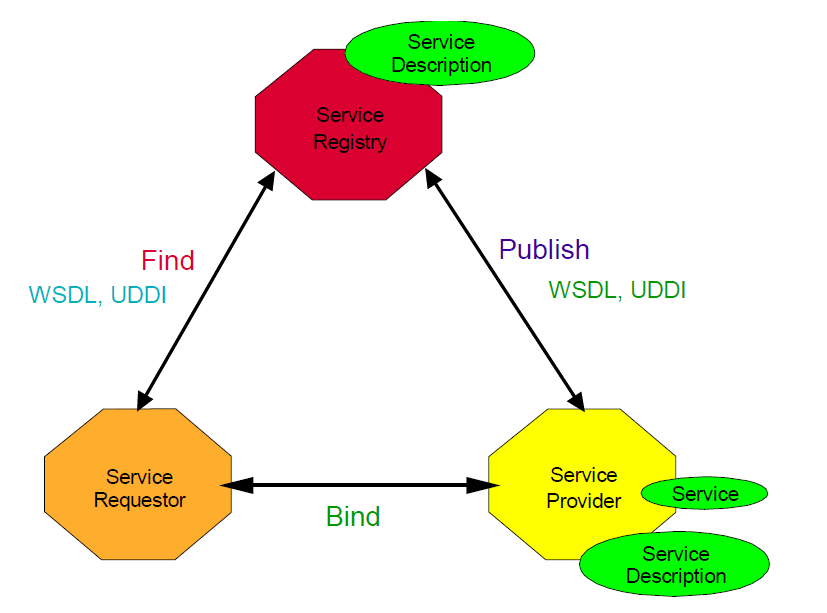
\includegraphics[width=\textwidth]{../images/background/ws_model.png}
	\caption{Web Services roles, operations and artifacts \cite{Kreger2001-WSC}}
	\label{fig:ws_model}
 \end{figure}
\end{center}

Service registry is a place where service providers can publish
descriptions of their services. Service requestors can find service descriptions
and get binding information from them. Binding can be static and dynamic.
Registry is needed more for dynamic binding where client can get service info at
the runtime, extract necessary functional methods and execute them on the
server. During static binding service description may be directly delivered to
the client at the development phase, for example using usual file, \gls{FTP}
server, Web site, email or any other file transfer protocol.
There are also available special protocols, named Service discovery protocols
(SDP), that allow automatic detection of devices and services on a network. One
of them is the \gls{UDDI} protocol, which is also was mentioned on
\autoref{fig:ws_model}. \gls{UDDI} is shortly described in
\nameref{sec:ws_protocol_stack} section.

\paragraph{\textbf{Artifacts of a Web Service}}
\newline
Web service consists of two parts~\cite{Kreger2001-WSC}:
\begin{itemize} 
\item \label{itm:service_description_artifact} 
\textbf{Service Description}~~~The
service description contains the details of the interface and implementation of the service. This includes its data types, operations, binding
information and network location. There could also be a categorization and
other metadata about service discovery and utilization. It may contain some
Quality of service (QoS) requirements. 

 \item \textbf{Service}
 ~~~This is the implementation of a service - a software module deployed on network accessible platforms provided by the service provider.
 Service may also be a client of other services. Implementation details
 are encapsulated inside a service, and client does not know the details how
 server processes his request.
\end{itemize}



\subsubsection{Web Services Protocol Stack}
\label{sec:ws_protocol_stack}

WS architecture uses many layered and interrelated technologies.
\autoref{fig:ws_protocol_stack} provides one illustration of some of these technology families.

\begin{center}
 \begin{figure}[h]
	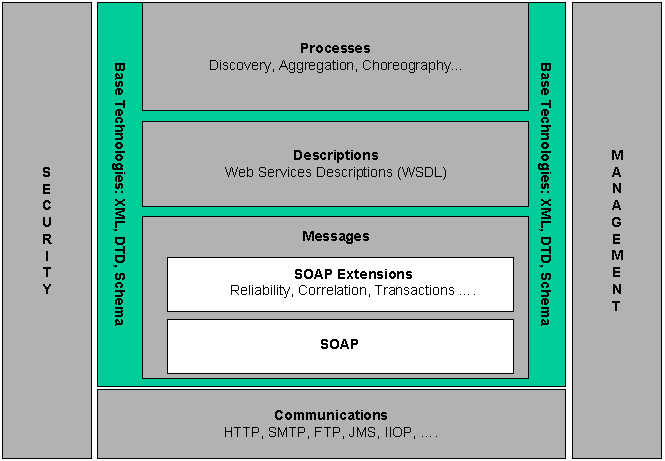
\includegraphics[width=\textwidth]{../images/background/ws_protocol_stack.png}
	\caption{Web Services Architecture Stack \cite{ws_arch} }
	\label{fig:ws_protocol_stack}
 \end{figure}
\end{center}

We can describe these different layers as follows:
\begin{itemize}
  \item \textbf{Communications} - This layer represents a transport between
  communication parties( service provider, client, service registry). This layer
  can be any network protocol like: \gls{HTTP}, \gls{FTP}, \gls{SMTP} or any
  other suitable transport protocol. If Web service is used in the Internet, the
  transport protocol in most cases will be \gls{HTTP}. In internal networks there is the opportunity to agree upon the use of alternative
network technologies.

\item \textbf{Messages} - In order to communicate with a service, client should
send a message. Messages are \gls{XML} documents with different structure.
\gls{SOAP} protocol defines how these messages should be structured.
\gls{SOAP} is implementation independent and may be composed using any
programming language. Protocol specification and message descriptions can be
found in document SOAP Version 1.2 Part 1: Messaging Framework (Second
Edition)\cite{soap_protocol_spec}.

\item \textbf{Descriptions} - This layer contains the definition of service
interface (see also \autoref{itm:service_description_artifact}). Web Services
use \gls{WSDL} language for describing the functionality offered by a service.
\gls{WSDL} file is the contract of service, which contains information about how
the service can be called, what parameters it expects, and what data structures it returns.
It is similar to method signatures in different programming languages.

\item \textbf{Processes} - This part contains specifications and protocols
about how service could be published and discovered. Web services are meaningful
only if potential users may find information sufficient to permit their execution.
Service as a software module has its own lifecycle, it needs to be deployed and deleted somehow.
Traditional Web Services use \gls{UDDI}  mechanism to register and locate web
service applications. \gls{UDDI} was originally proposed as a core Web service
standard.

\item \textbf{Security} - Threats to Web services include threats to the host
system, the application and the entire network infrastructure. To solve problems
like authentication, role-based access control, message level security there is
need for a range of XML-based security mechanisms.

Web services architecture uses WS-Security\footnote{WS-Security (Web Services
Security, short WSS) is an extension to SOAP to apply security to web services.
It is a member of the WS-* family of web service specifications and was
published by OASIS(Organization for the Advancement of Structured Information
Standards, https://www.oasis-open.org/). \cite{wikipedia:WS-Security}}
~protocol to solve security problems.
This protocol specifies how \gls{SOAP} messages may be secured.
 


\item \textbf{Management} -
Web service management tasks are~\cite{ws_arch}: monitoring, controlling,
reporting of service state information. 

Web services architecture uses WS-Management~\cite{ws_security_promo} protocol
for management of entities such as PCs, servers, devices, Web services and other
applications. WS-Management has ability to discover the presence of management resources,
control of individual management resources, subsrcibe to events on resources,
execute specific management methods.

WS-Management was created by DMTF( Distributed Management Task Forse, Inc.,
http://www.dmtf.org/) organization, which is creating stantards for managing
the enterprise level systems. Organisation members are largest hardware and
sortware corporations like Broadcom, Cisco, Fujitsu, Hewlett-Packard, IBM, Intel,
Microsoft, Oracle. DTMF standards promote multi-vendor interoperability, which
is great for the integration between different IT systems. 

\end{itemize}

Most of mentioned protocols are recommended by W3C Consortium and are production
standards. Lots of \gls{SOA} information systems use WS-* protocols for
enterprise level services. Mostly these protocols are based on \gls{XML} and
\gls{SOAP}. One example of such protocol is the \gls{WSDL} service description.

\subsubsection{Service Description and Service Contract}
\label{sec:ws_service_contract}
\gls{WSDL} file is an \gls{XML} document which has specification of  service contract.
As it was mentioned earlier(\autoref{itm:service_description_artifact}) contract should be shipped with a component and should  tell the
client what input does service expect, and what output it will produce if specified input conditions are met. 
Contract may be a primary specification and it should be enough for a client to start using a service.
This is similar to library header file in C language. 
You have a ready and compiled library shipped with a header file, where are all
method declarations and definitions of data structures.
If header file is verbose enough, there is no need to use the documentation. You can place this component into your system very easily.



Regular \gls{WSDL} document contains some necessary elements
~\cite{wsdl_language_spec, wikipedia:WSDL}: Service, Endpoint, Binding,
Interface and Message Types. \autoref{tbl:wdsl_members} describes them in
details.


\begin{table}[h]
	\centering	
	\begin{tabular}[h]{|l|p{10cm}|}
		\hline
		\textbf{WSDL 2.0 Term} & 
		\textbf{Description} 	
	    	\tabularnewline
		\hline
			Service &
			The service element describes \textit{where} to access the service.\newline A
			WSDL 2.0 service specifies a single interface that the service will support,
			and a list of endpoint locations where that service can be accessed.
	    	\tabularnewline	    	
	    	\hline
			Endpoint & 
			Defines the address or connection point to a Web service.
			It is typically represented by a simple HTTP URL string.			
			Each endpoint must also reference a previously defined binding to indicate			
			what protocols and transmission formats are to be used at that endpoint.				
	    	\tabularnewline

	    	\hline
			Binding &		
			Specifies concrete message format and transmission protocol details			 
			for an interface, and must supply such details for every operation			 
			and fault in the interface.
	    	\tabularnewline

	    	\hline
			Interface &
			Defines a Web service, the operations that can be performed,			
			and the messages that are used to perform the operation.			
			Defines the abstract interface of a Web service as a set of abstract \textit{operations},			
			each operation representing a simple interaction between the client and the service.			
			Each operation specifies the types of messages that the service can send or receive as part of that operation.			
			Each operation also specifies a message exchange \textit{pattern} that indicates the sequence in which the associated messages are to be transmitted between the parties. 
	    	\tabularnewline

		\hline
			Message Types &
			The types element describes the kinds of messages that the service will send and receive.			
			The XML Schema\footnotemark ~language (also known as XSD) is used (inline or
			referenced) for this purpose.
	    	\tabularnewline
		\hline	  
	\end{tabular} 
	\caption{Objects in WSDL 2.0~\cite{wsdl_language_spec, wikipedia:WSDL} }
	\label{tbl:wdsl_members}
\end{table}
 
\footnotetext{XML schema is the XML document, that
			specifies structure of other XML document and describes data types and constraints, that other document might have. 
			You can create a schema for necessary XML data structure and verify if processed message corresponds to schema you have already defined}


Document may also contain optional element named \textit{documentation}.
There may be human readable service documentation, with   purpose and use of the service, the meanings of all messages, constraints their use, and the sequence in which operations should be invoked.
To be documentation more complete, you may specify an external link to any additional documentation.


You can see the example of WSDL service contract in the appendix 
\autoref{sec:appendix_service_contracts}. This example is from the official
\gls{WSDL} standard ~\cite{wsdl_language_spec}. It describes a hotel reservation
service, where you can book you a room in a fictional hotel named GreatH. For simplicity it describes
only one method - the \textit{opCheckAvailability} operation. This description
is quite verbose to understand what it is about. There is input and output
object type declaration. It also has an output error response declaration and
if some error occures during client request processing, server should send a
message of specified kind.
These \gls{XML} object types are declared in different \textit{namespaces} ( see
xmlns:*	declarations at the start of \gls{WSDL} document). This gives an ability
to group domain types into one separate file and your main description
file would not be overcrowded.


\gls{WSDL} definition of the service does not contain any additional
information about service hosting company and its products. At the moment when
you get a service contract, you already know what company provides this service and what
for this service was made. There is assumption that service provider somehow
gave you this service contract. Another possibility to get the service
description is to use a special \textit{directory} or catalog, where you can
find all information about company you are dealing with. Web Services
architecture include \gls{UDDI} mechanism for that particular purpose.

Official \gls{UDDI} Version 3.0.2 Technical Specification draft~\cite{uddi_spec}
defines \gls{UDDI} as follows:
\begin{quotation}
\textit{
 The focus of Universal Description Discovery & Integration (UDDI) is the
definition of a set of services supporting the description and discovery of (1) businesses,
organizations, and other Web services providers, 
(2) the Web services they make available,
 and (3) the technical interfaces which may be used to access those services.
 Based on a common set of industry standards, including HTTP, XML, XML Schema, and SOAP,
 UDDI provides an interoperable, foundational infrastructure for a Web services-based software environment
 for both publicly available services and services only exposed internally within an organization.
}
\end{quotation}

\gls{UDDI} mechanism uses \gls{SOAP} messages for client-server communication. 
Service provider publishes the \gls{WSDL} to \gls{UDDI} registry and client can
find this service by sending messages to the registry ( see also 
\autoref{fig:ws_model}). \gls{UDDI} specification defines the communication
protocol between \gls{UDDI} registry and other parties.


\gls{UDDI} registry is a storage directory for various service contracts, where
lots of companies hold their service descriptions. \gls{WSDL} contracts may 
also be published on a company website using direct link to the \gls{WSDL} file,
but \gls{UDDI} contains them all in one place with the ability to search and
filter.
You have a choice and there is a possibility to find most suitable service
from all provided companies and services.



\subsubsection{Advantages and disadvantages of WS-* standards}
Usage of WS-* technologies gives some
benefits~\cite{ws_techologies_state_of_the_art}:

\begin{itemize}
  \item Reusability
  \item Interoperability and Portability
  \item Standardized Protocols
  \item Automatic Discovery
  \item Security
\end{itemize}

WS-* uses the \gls{HTTP} protocol as transport medium for exchanging messages
between web services. \gls{SOAP} messages can be transfered using another
protocol (\gls{SMTP}, \gls{TCP}, or \gls{JMS}), which can be more suitable to
your system environment than \gls{HTTP}.

One another fundamental characteristic of web services is the service
description and contract design. Contract specification gives you the ability to
reuse service functionality in many different and separate applications.
Contract in Web Services is general standardized description of a service in
universal data format (\gls{XML} and \gls{WSDL}), that is platform and programming language
independent. Service description is only the interface and the implementation
of that interface may be unknown by the service client. There is possibility to
transparently change (totally or partially) implementation details of a service.


The main reason why Web Services standards are bad in context of embedded
systems is the performance.
Web services impose additional overhead on the server since they require the
server to parse the \gls{XML} data in the request. Web Services use \gls{SOAP}
messages, which are structured \gls{XML} data, for client-server communication.
Some experiments~\cite{1182978, 5470528} show that performance of SOAP transfer
is more than 5 times slower compared to others \gls{SOA} implementations, like
CORBA~\footnote{The Common Object Request Broker Architecture (CORBA) is a
standard defined by the Object Management Group (OMG) that enables software
components written in multiple computer languages and running on multiple
computers to work together (i.e., it supports multiple
platforms).\cite{wikipedia:CORBA}} or custom made protocol messages. If you
start reading WS-* standarts one by one, you will ensure that all they are
interconnected using idea of \gls{XML}, \gls{SOAP} and \gls{HTTP}. 


Another statement against Web Services is that these standards are too
complicated and their documentation is hard to
understand. Document ~\cite{dguinard-rest-vs-ws} contains a use case survey
about two most common implementations of SOA: Web Services and \gls{REST}. Most of people
in the survey agreed that WS-* standards is not easy to learn and adapt. WS-*
suits better for highly integrated business solutions, but not for simple
applications, with atomic functionality.

WS-* standarts rely on each other and to implement a small web service with
few features you will need to dive into all WS standards. This is at least 783
pages of not just text, but a techical specifications~\cite{ws_pagecount}.
Surely, Web services have good ideas, but this technology is promoted and
developed by large corporations like Microsoft, IBM, Oracle, who are not
intrested in simple and lightweight solutions, because they need to utilize
their thousands of developers and earn money( document ~\cite{ws_pagecount} says
that most of WS-* specifications are hosted by Microsoft and  OASIS
organisation, which foundational sponsors are IBM and Microsoft).
It seems that Web services are trying to solve every business problem and there
is a \textit{WS-problem} standart for it.


This topic described Web Service architecture features. There are lots of
useful principles like portability, interface description and message exchange
patterns, but the WS-* implementation is not suitable for resource-constrained
hardware.


The \gls{REST} has some advantages over WS-*. Next section will shortly
describe the main principles of \gls{REST} approach. 





